\chapter{INI3KX.}

\begin{figure}[h!]
\centering

\includegraphics[width=0.8\textwidth]{../imagenes/pagina_016_fig_01.png}
\caption{Figura de la página 16}
\end{figure}

\begin{figure}[h!]
\centering

\includegraphics[width=0.8\textwidth]{../imagenes/pagina_016_fig_02.png}
\caption{Figura de la página 16}
\end{figure}

ACCIDENT NO. I, 26. of, 93. AUDIBLE SOUND, GUSHER, limited to twelve inches the, 285. of the violin sounding- HARMONICS, board, 53. HARMONICOVER- value of, 96. ANGLES, incidence and reflection, TONES, 294. 304. INTRODUCTION XII, BOOKS, method of arriving at unreliable evidence in, conclusions, xiv, eight 35. propositions, xv. BEST SOLO VIOLIN, INANITY, not best orchestra vio- continuing the demand lin, 37. that soloists only appear BACK PLATE, with a Stradivarius, or functions of, 47; as a Guarnerius, 39. tone-producing agent, INVITATION, 107. to my sheep-herder vio- CARE OF VARNISH, lin, 101. example, 93. LONGEVITY CREMONA VARNISH, of the violin, 98; exam- 125. ple, 98. COMBINED TONAL EF- LOSS OF TONE-POWER, FECT, causes of, 299. half dozen violins of METEORICCONDI- uniform tone-pitch, 136. conditions of test, 136. TIONS, 23. COLD TONE, 296. Musical sound, explicit DISSONANTOVER- law, 30; affecting dis- tance traveled by violin TONES, tone, 280. cause of, 30; 295. MAXIMUM EVENNESS FRAUD, 43. GENERAL PURPOSE of violin tone-power, 205; fundamental tones, Violin, 38. 208; reasons leading to GUMS, a new method for sound- hard, inelastic, eifect ing-board graduation,

\section{vin}

\begin{figure}[h!]
\centering
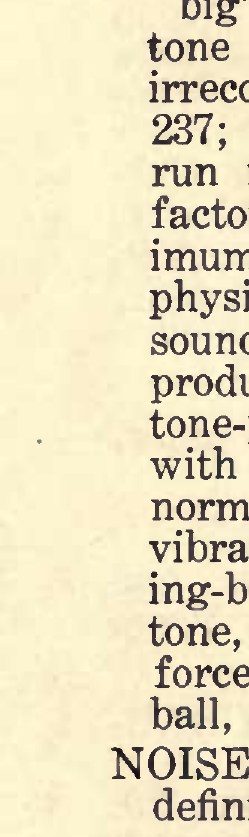
\includegraphics[width=0.8\textwidth]{../imagenes/pagina_017_fig_01.png}
\caption{Figura de la página 17}
\end{figure}

INDEX. 214; demonstration of PLAYERS, sounding-board areas Varying opinions of, 36. augmenting tone of each PHILOSOPHY string, 216; ratio for Involved in violin in- lengths of fiber-activi- terior-surface condit- ty beneath each string, ions, 256; list of princi- 218; concert pitch 200 pals modifying violin years ago, 223; demon- tone, 259; number of stration that errors in tone-qualities absolute- sounding-board gradua- ly at command of the tion cause uneven tone- violin builder, 261; in- power, 225. tensity of violin-tone MAXIMUM TONE-POW- the product of four fac- ER, 235; tors, 262; properties of "big" tone, 236; violin air affecting intensity tone separated by two of violin tone, 264. irreconcilable factors, PENETRATION 237; violin aestheticism of 274. run mad, 238; list of PASS-OVER, oil, factors producing max- 276. imum violin tone-power; POST, physical appearances of problem of, 301. sounding-board wood POST-SETTING, 303. producing maximum RICH TONE, tone-power combined causes of, 96; descrip- with "rich" tone, 246; tion of wood yielding normal and transverse rich tone, 97; illustra- vibration in the sound- tion, 296. ing-board, 249; woody SCIENCE, tone, 255; dispersion of never made a violin, 32. force, the rebounding SCIENTIFIC STATE- ball, 271. MENTS, NOISE, received with caution 32 definition of, 25. SOUNDING-BOARD NODES, 294. WOOD, 57; 0, THOU POST, 276. mite contributed by sci- PITCH, ence, 58; value in scru- Musical sound, 30. tinizing wood of used\\
IX\\